%
\documentclass[tikz,border=10pt]{standalone}
\usetikzlibrary{calc,intersections,backgrounds}
%
\tikzset{
axes/.style = {line width = 1.pt},
grid/.style = {line width = 0.5pt,color = gray}
}
%
\begin{document}
%
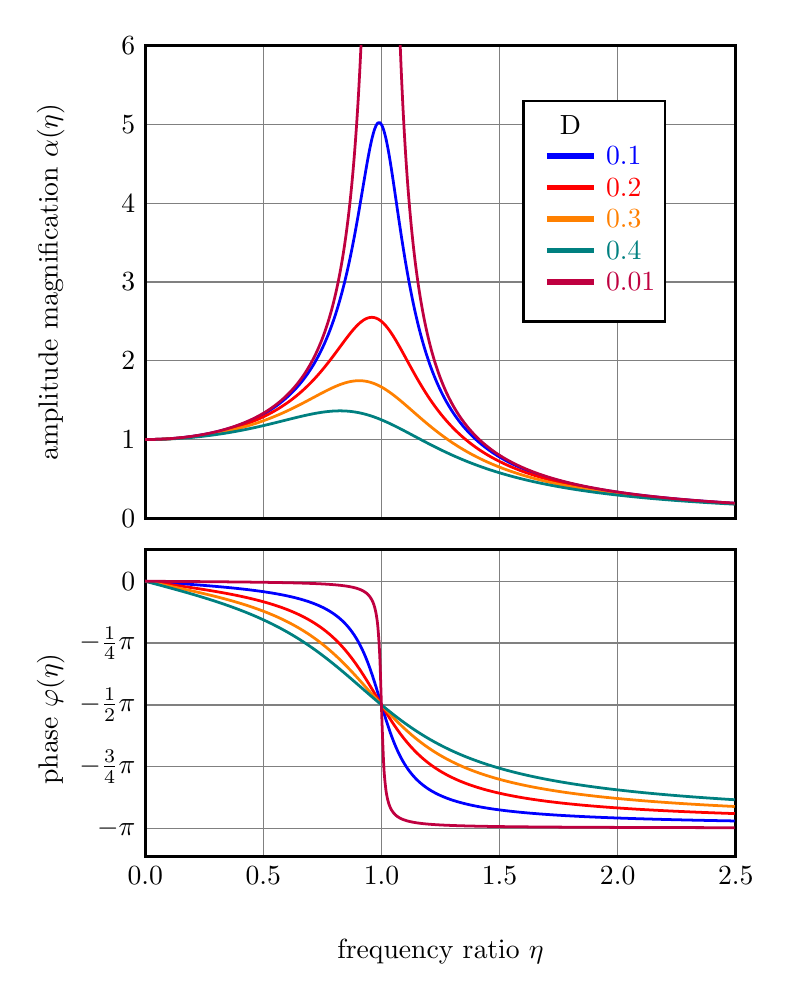
\begin{tikzpicture}
%
\def\Dlist{0.1,0.2,0.3,0.4,0.01}
\def\colorlist{{"blue","red","orange","teal","purple"}}
\def\xlist{0.0,0.5,1.0,1.5,2.0,2.5}
\def\ampylist{0,1,2,3,4,5,6}
\def\phaseylist{0/0,-0.25*3.14/$-\frac{1}{4}\pi$,-0.5*3.14/$-\frac{1}{2}\pi$,-0.75*3.14/$-\frac{3}{4}\pi$,-3.14/$-\pi$}
%
\def\xmax{2.5}
\def\ymax{6}
\def\ymin{-3.5}
\def\pos{0.8cm}
\def\tagshift{1.2cm}
\def\xsc{3}
%
\begin{scope}[xscale=\xsc]
%
\foreach \x in \xlist {
\draw[grid](\x,0)--(\x,\ymax);
\draw[grid,yshift=-\pos](\x,\pos/2)--(\x,\ymin);
\node[yshift=-\pos, anchor = north] at (\x,\ymin){\x};
}
%
\foreach \y in \ampylist{\draw[grid](0,\y)--(\xmax,\y)node[at start, left, color = black]{\y};}
\foreach \y/\tag in \phaseylist{\draw[grid,yshift=-\pos](0,\y)--(\xmax,\y)node[at start, left, color = black]{\tag};}
%
%
\draw[axes](0,0)rectangle(\xmax,\ymax);
\draw[axes,yshift=-\pos] (0,\pos/2)rectangle(\xmax,\ymin);
%
\draw[fill=white,draw=black,line width=1pt] (1.6,5.3) rectangle (2.2,2.5);
\node[] at (1.8,5){D};
%
\foreach \D [count=\i] in \Dlist {
\pgfmathsetmacro{\c}{\colorlist[\i-1]}
\begin{scope}
\clip[](0,0) rectangle (\xmax,\ymax);
\draw[domain=0:\xmax,samples=300,smooth,variable=\x,line width = 1pt,color=\c] plot (\x,{sqrt(1/((2*\D*\x)^2+(1-\x^2)^2))});
\end{scope}
%
\draw[yshift=-\pos,domain=0:\xmax,samples=300,smooth,variable=\x,line width = 1pt,color=\c] plot (\x,{3.14/180*atan2(-2*\D*\x,1-\x^2)});
%
\draw[line width = 2pt,color=\c] (1.7,5-\i*0.4)--(1.9,5-\i*0.4)node[at end,right]{\D};
%
}
%
\node[rotate=90] at($(0,\ymax/2)+(-\tagshift/\xsc,0)$){amplitude magnification $\alpha(\eta)$};
\node[yshift = -\pos,rotate=90] at($(0,\ymin/2)+(-\tagshift/\xsc,0)$){phase $\varphi(\eta)$};
\node[yshift = -\pos] at($(\xmax/2,\ymin)+(0,-\tagshift)$){frequency ratio $\eta$};
%
\end{scope}
%
\end{tikzpicture}
%
\end{document}
%